\chapter{Evaluation}
\label{ch:evaluation}
In diesem Kapitel wird die Leisungsfähigkeit der Implementierung mit Hilfe verschiedener Benchmarks und Vergleiche untersucht.

\begin{table}[h]
	\centering
	\caption{Eigenschaften der Szenen}
	\label{tbl:local_scenes}
	\begin{tabular}{|c|c|c|c|c|c|}
		\hline
		Szene 			& Auflösung & Dreiecke	& Lichtquellen & Rekursiontiefe & Samples \\ \hline
		Cube  			& 8000x6000 & 12 	& 2	& -	& -			\\
		Sponza  		& 2048x2048 & 262267 	& 1 & -	& -			\\
        Cornell (PT) 	& 800x600 & 14 	& 8			& 1	& 4000	\\
		Sponza (PT) 	& 400x400 & 262267 & 12			& 1	& 32	\\
		\hline
	\end{tabular}
\end{table}

\begin{table}[h]
	\centering
	\caption{Laufzeiten der lokalen Benchmarks}
	\label{tbl:local_bench}
	\begin{tabular}{|c|c|c|c|c|c|c|}
		\hline
		Szene 			& naiv		& k-d-Baum	& + AVX		& + SAH		& GPU 		& Heuristik \\ \hline
		Cube  			& 00:03:84 	& 00:03:73  & 00:03:42	& 00:03:21	& -			& 00:03:50	\\
		Sponza  		& $\infty$ 	& 01:41:17 	& 00:21:51  & 00:06:79	& -			& 00:06:38	\\
		Cornell (PT) 	& $\infty$ 	& 01:22:01 	& -			& 01:25:76	& 00:22:31	& 00:20:05	\\
		Sponza (PT) 	& $\infty$ 	& 07:17:73	& -			& 00:17:84	& 01:29:12	& 00:17:71	\\
		\hline
	\end{tabular}
\end{table}

\section{Hauptspeicher}
Für eine Szene mit 262267 Primitiven wird während des kompletten Renderprozesses ungefähr 1GB Hauptspeicher benutzt. Soll die Szene auf der GPU berechnet werden, wird geprüft, ob die zu benutzende GPU über genug Speicher verfügt. 

\section{Laufzeit}
Die Implementierung wurde auf den Praktikumssystemen sowie auf einer Enticklungsmaschine (im Folgenden \glqq lokaler Benchmark\grqq) in der Laufzeit evaluiert. Die lokalen Benchmarks wurden auf einem System mit Ubuntu 16.04, Intel Core i5-6600K CPU @ 3.50GHz, 32 GB Hauptspeicher und einer Nvidia Geforce GTX 1070 Grafikkarte mit 8 GB Grafikspeicher ausgeführt.  In Tabelle \ref{tbl:local_bench} sind die Zeiten des lokalen Benchmarks aufgelistet. Getestet wurden vier verschiedene Szenen (Cube, Sponza, Cornell-Box mit Pathtracing und Sponza mit Pathtracing). In Tabelle \ref{tbl:local_scenes} sind die Eigenschaften der Benchmarkszenen gelistet. Bei Pathtracing handelt es sich um Flächenlichtquellen. Das heißt es gibt Flächen die Licht emittieren und keine gesonderten Punktlichtquellen. Verglichen werden naive Implementierung (vollständige Suche), k-d-Baum, k-d-Baum mit AVX-Strahlbündelschnitt, selbiger mit SAH-Heuristik und für die Pathtracing-Szenen das Rendern auf der GPU (Nutzung des trivialen k-d-Baumes). Die Spalte Heuristik zeigt die erreichten Zeiten, wenn die Implementierung Datenstruktur und Ausführungsumgebung selbst wählt. Alle Benchmarkes wurden OpenMP-parallelisiert ausgeführt.

Nachfolgend sind die Ergebnisse der Benchmarks der Wettbewerbsmaschinen zu sehen. In Abbildung \ref{img:ptnormal} sind die Ergebnisse mit dem Pathtracing Algorithmus aus \cite{Kajiya:1986:RE:15886.15902} zu sehen und in \ref{img:ptdiffuse} sind die Ergebnisse mit dem vorgegebenen Algorithmus zu sehen.

\begin{figure}[htbp]
	\centering
	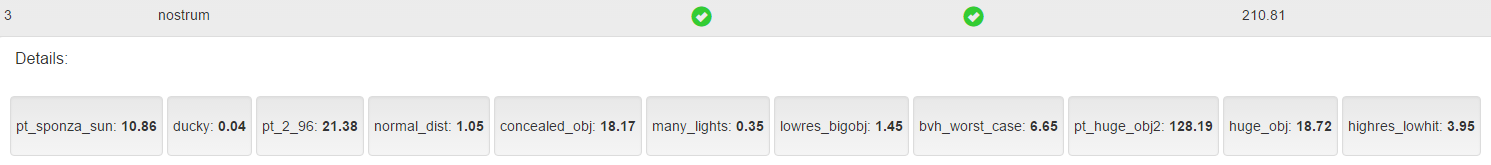
\includegraphics[width=1\textwidth]{graphics/nostrum_benches_avx_nogpu_ptnormal.PNG}
	\caption{Wettbewerbsmaschine \textit{i41pc189}: Pathtrace Algorithmus aus \cite{Kajiya:1986:RE:15886.15902}}
	\label{img:ptnormal}
\end{figure}

\begin{figure}[htbp]
	\centering
	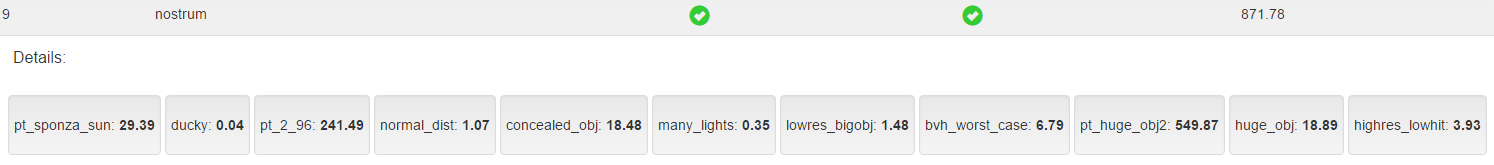
\includegraphics[width=1\textwidth]{graphics/nostrum_benches_avx_nogpu_ptdiffuse.PNG}
	\caption{Wettbewerbsmaschine \textit{i41pc189}: Vorgegebener Pathtrace Algorithmus}
	\label{img:ptdiffuse}
\end{figure}
